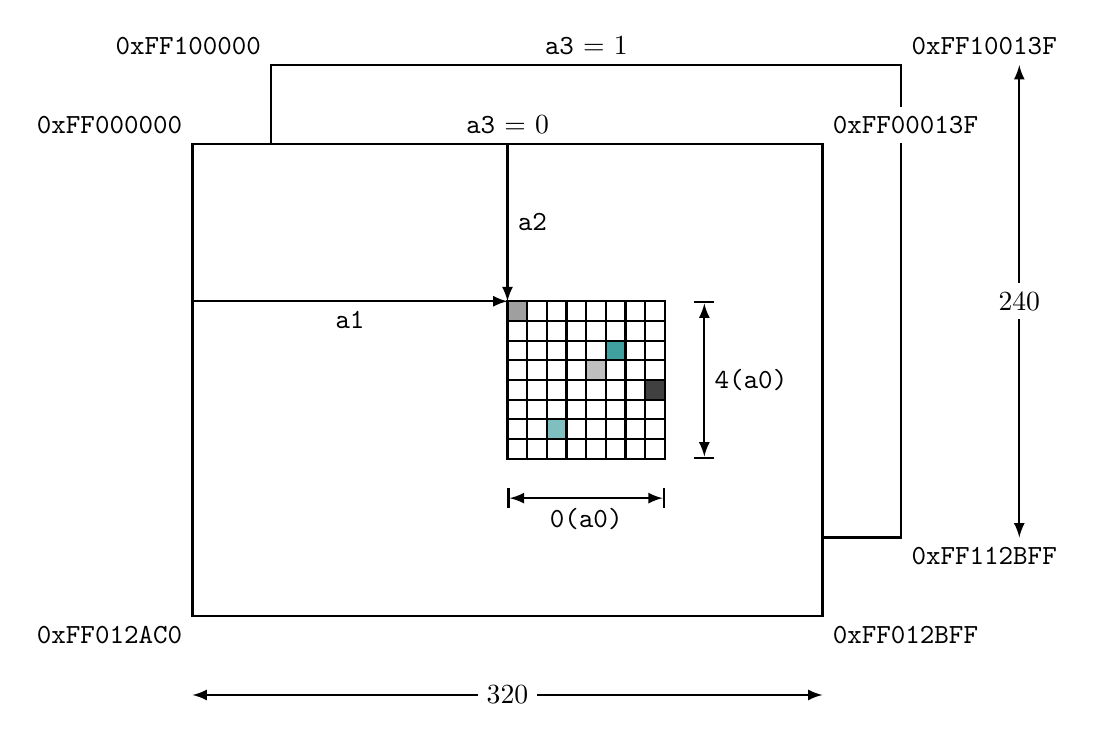
\begin{tikzpicture}[>=latex, thick]
    % frame 1
    \begin{scope}[shift={(1,1)}]
        \draw (0, 0) rectangle (8, 6);
        \draw
            node (FF100000) at (0, 6) {}
            node (FF10013F) at (8, 6) {}
            node (FF112BFF) at (8, 0) {}
            node (FF112AC0) at (0, 0) {}
        ;
        \draw 
            (FF100000.center) node [above left] {{\tt 0xFF100000}}
            (FF10013F.center) node [above right] {{\tt 0xFF10013F}}
            (FF112BFF.center) node [below right] {{\tt 0xFF112BFF}}
            %(FF112AC0.center) node [below left] {{\tt 0xFF112AC0}}
        ;
        \draw [<->] 
            (9.5, 6) --++ (0, -6) node [midway, fill=white] {240}
        ;
        \draw (4, 6) node [above] {{\tt a3} = 1};
    \end{scope}

    % frame 0
    \draw [fill=white] (0, 0) rectangle (8, 6);
    \draw
        node (FF000000) at (0, 6) {}
        node (FF00013F) at (8, 6) {}
        node (FF012BFF) at (8, 0) {}
        node (FF012AC0) at (0, 0) {}
        
        (FF000000.center) node [above left] {{\tt 0xFF000000}}
        (FF00013F.center) node [above right, fill=white] {{\tt 0xFF00013F}}
        (FF012BFF.center) node [below right] {{\tt 0xFF012BFF}}
        (FF012AC0.center) node [below left] {{\tt 0xFF012AC0}}
    ;
    \draw [<->] 
        (0, -1) --++ (8, 0) node [midway, fill=white] {320}
    ;
    \draw [->] 
        (0, 4) --++ (4,0) node [midway, below] {\tt a1}
    ;
    \draw [->] 
        (4, 6) --++ (0,-2) node [midway, right] {\tt a2}
    ;
    \draw [|<->|] 
        (6.5, 4) --++ (0,-2) node [midway, right] {\tt 4(a0)}
    ;
    \draw [|<->|] 
        (4, 1.5) --++ (2,0) node [midway, below] {\tt 0(a0)}
    ;
    %% algumas cores
    \fill   [gray!50]   (5, 3) rectangle +(0.25, 0.25);
    \fill   [gray!75]   (4, 3.75) rectangle +(0.25, 0.25);
    \fill   [gray!50!black]   (5.75, 2.75) rectangle +(0.25, 0.25);
    \fill   [teal!50]   (4.5, 2.25) rectangle +(0.25, 0.25);
    \fill   [teal!75]   (5.25, 3.25) rectangle +(0.25, 0.25);
    %% grade
    \draw (4, 4) rectangle +(2, -2);
    \foreach \i in {4, 4.25, 4.5, ..., 5.75} {
        \draw 
            (\i, 2) --++ (0,2)
            (4, \i-2) --++ (2,0)
        ;
    }
    \draw (4, 6) node [above] {{\tt a3} = 0};
\end{tikzpicture}